\chapter{Campaign and Analysis}
\label{campaign_and_analysis}
The analysis of this campaign is based on the observation campaign of NGC4593 in 2016 by Edward M. Cackett \parencite{cackett2018accretion}. This campaign took place between the 12th of July and the 6th of August with daily observations, which resulted in 26 successful out of 27 observations. It was performed with the Hubble Space Telescope (HST) using the Space Telescope Imaging Spectrograph (STIS) with the three different Gratings. The following section will cover an overview of the properties and specifications of NGC4593 and the campaign in 2016.

\section{NGC4593}
\label{NGC4593}

NGC 4593 is an active galactic nucleus (AGN), classified as a Seyfert 1 galaxy with a \mbox{(R)SB(rs)b} barred spiral morphology. 
It is located in the southern sky at RA = 12:39:39.44, DEC = $-05$°$ 20' 39.03''$ (J2000) and has a redshift of $z = 0.0083 \pm 0.0005$, corresponding to a distance of about $35.6$ Mpc \parencite{simbaNGC4593} based on the $\Lambda$CDM model. 
The galaxy exhibits a prominent large-scale bar and nuclear dust ring connected to dust lanes along the bar, which likely channel gas toward the central region \parencite{mulchaey1997structure}, as seen in figure \ref{fig:NGC4593}. ALMA observations, conducted by \parencite{garcia2019alma}, reveal a central molecular gas reservoir of $\sim 10^8 \ M_\odot$ arranged in a one armed spiral and a circumnuclear ring, as well as evidence for a mild molecular outflow on scales of a few hundred parsecs, highlighting the interplay between a bar driven inflow and an AGN feedback in this galaxy. Luminosity: https://simbad.u-strasbg.fr/simbad/sim-id?Ident=NGC++4593

\begin{figure}[!ht]
	\centering
	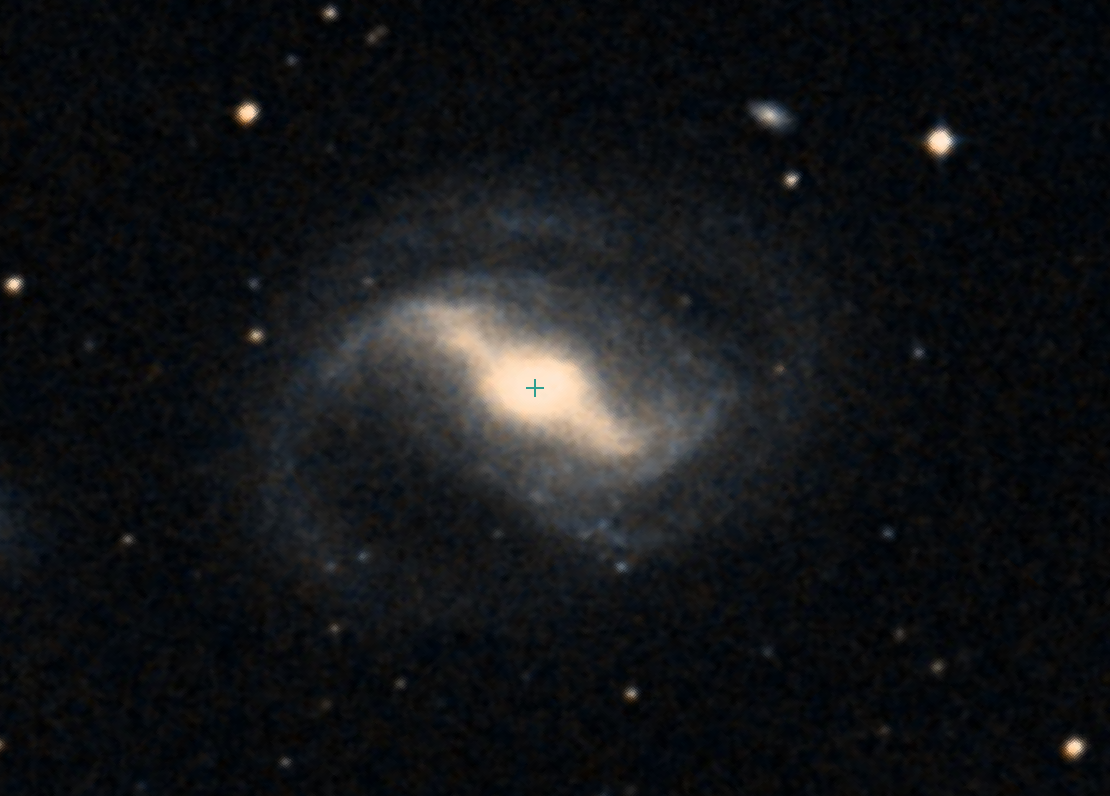
\includegraphics[width=0.55\textwidth]{pictures/Chapter3/NGC4593.PNG}
	\caption{A DSS image of NGC4593.}
	\label{fig:NGC4593}
\end{figure}

\newpage
The AGN of NGC4593 shows strong broad emission lines in  H$\alpha$,  H$\beta$,  H$\gamma$, Ly$\alpha$, He\,\textsc{i}, and He\,\textsc{ii} \parencite{bentz2015agn}, indicating a well-developed broad-line region. Earlier reverberation mapping campaign based these broad lines showed a supermassive black hole mass of about $M = \left(7.63 \pm 1.62\right) \times 10^6\,M_\odot$ \parencite{bentz2015agn}, which corresponds to a broad-line region radius of only a few light-days \parencite{denney2006ngc4593}. Furthermore NGC4593 shows strong variability from X-ray to optical bands, with time delays that indicate a UV/optical-emitting accretion disk about three times larger than predicted by standard thin-disk theory and signatures of diffuse continuum emission from the BLR \parencite{cackett2018accretion}. 


\section{2016 Campaign by E. M. Cackett}
\label{Campaign_Cackett}

E. M. Cackett's campaign was designed to study wavelength dependent continuum lags. Therefore, the STIS instrument on the Hubble Space Telescope was used with low-resolution gratings to measure a broad range of wavelengths. In each observation, spectra were taken using three different gratings: G140L, G430L, and G750L. These were used together with the $52'' \times 0.2''$ slit.\\
The characteristics of the STIS gratings used in this analysis are summarized in Table \ref{tab:stis_gratings}. After a standard pipeline-processing, a package was used to do a Charge Transfer Inefficiency correction with an algorithm based on \parencite{anderson2010empirical}. The few left rest of hot pixels got manually removed by interpolating the flux of neighbor pixels.\\


\begin{table}[h!]
	\centering
	\small
	\caption{Overview of STIS Grating Characteristics \parencite{stisgratings}}
	\label{tab:stis_gratings}
	\begin{tabular}{lcccc}
		\hline
		\textbf{Grating} & \textbf{Range [\AA]} & \textbf{Exp. Time [s]} & \textbf{Res. Power} & \textbf{Dispersion [\AA/pixel]} \\
		\hline
		G140L  & 1119--1715  & 1234 & $\sim 1000$         & 0.6 \\
		G430L  & 2888--5697  & 298  & $\sim 500 - 1000$    & 2.73 \\
		G750L  & 5245--10233 & 288  & $\sim 500 - 1000$    & 4.92 \\
		\hline
	\end{tabular}
\end{table}

\newpage


\section{Intercalibration and Determination of AVG and RMS Spectra}

Reverberation mapping requires multiple epochs to capture variability. For the 2016 campaign of NGC 4593, we retrieved 27 spectra from the ... archive of which 26 are usable for further analysis. The top panel of Figure \ref{fig:comparison_spectra} shows a section between about $4000\,\text{\AA}$ and $9000\,\text{\AA}$ of the optical spectral range from these epochs.\\
For the subsequent analysis, the average spectrum (AVG) is obtained by averaging over all epochs. Ideally, this improves the signal-to-noise ratio (S/N) sufficiently to identify spectral features in NGC 4593.  Furthermore it is essential for the reverberation mapping analysis to identify variability between the epochs, which can be obtained with the root-mean-spuare (RMS) spectrum, defined as the standard deviation of the flux at each wavelength across epochs:
\begin{equation}
	F_{\mathrm{RMS}}(\lambda) = \sqrt{\frac{1}{N-1}\sum_{i=1}^{N}\left[F_i(\lambda)-\bar{F}(\lambda)\right]^2}\,,
\end{equation}
with the mean spectrum at wavelength $\lambda$ given by
\begin{equation}
	\bar{F}(\lambda) = \frac{1}{N}\sum_{i=1}^{N} F_i(\lambda)\,.
\end{equation}

Constant features, like narrow emission lines, vanishes in the RMS spectrum, whereas variable components, like broad emission lines stands out. The top panel of Figure \ref{fig:comparison_spectra_avg_rms} shows the AVG and RMS spectra from the original retrieved data. It showes, that residual variability remains in nominally non-varying lines, especially in the forbidden features near $5000\,\text{\AA}$. This indicates small wavelength misalignment between epochs. Therefore an intercalibration anchored to the narrow [O \textsc{iii}] $\lambda5007$ line was performed. The lower panels of Figures \ref{fig:comparison_spectra} and \ref{fig:comparison_spectra_avg_rms} present the intercalibrated epochs and the corresponding AVG and RMS spectra. The disappearance of narrow features in the calibrated RMS spectrum confirms that the apparent variability in the uncalibrated RMS was induced by the wavelength shifts between the epochs rather than intrinsic line variability. However the intercalibration was only applied to the optical part of the spectra  due to its limited reliability. Following that the intercalibrated AVG and RMS spectra will be used for optical part, taken by the G430L and G750L gratings used in the following analysis and the uncalibrated AVG and RMS spectra for the emission lines in the UV part of spectrum and their analysis, as they were taken by the G140L gratings. 
\newpage
\begin{figure}[!ht]
	\centering
	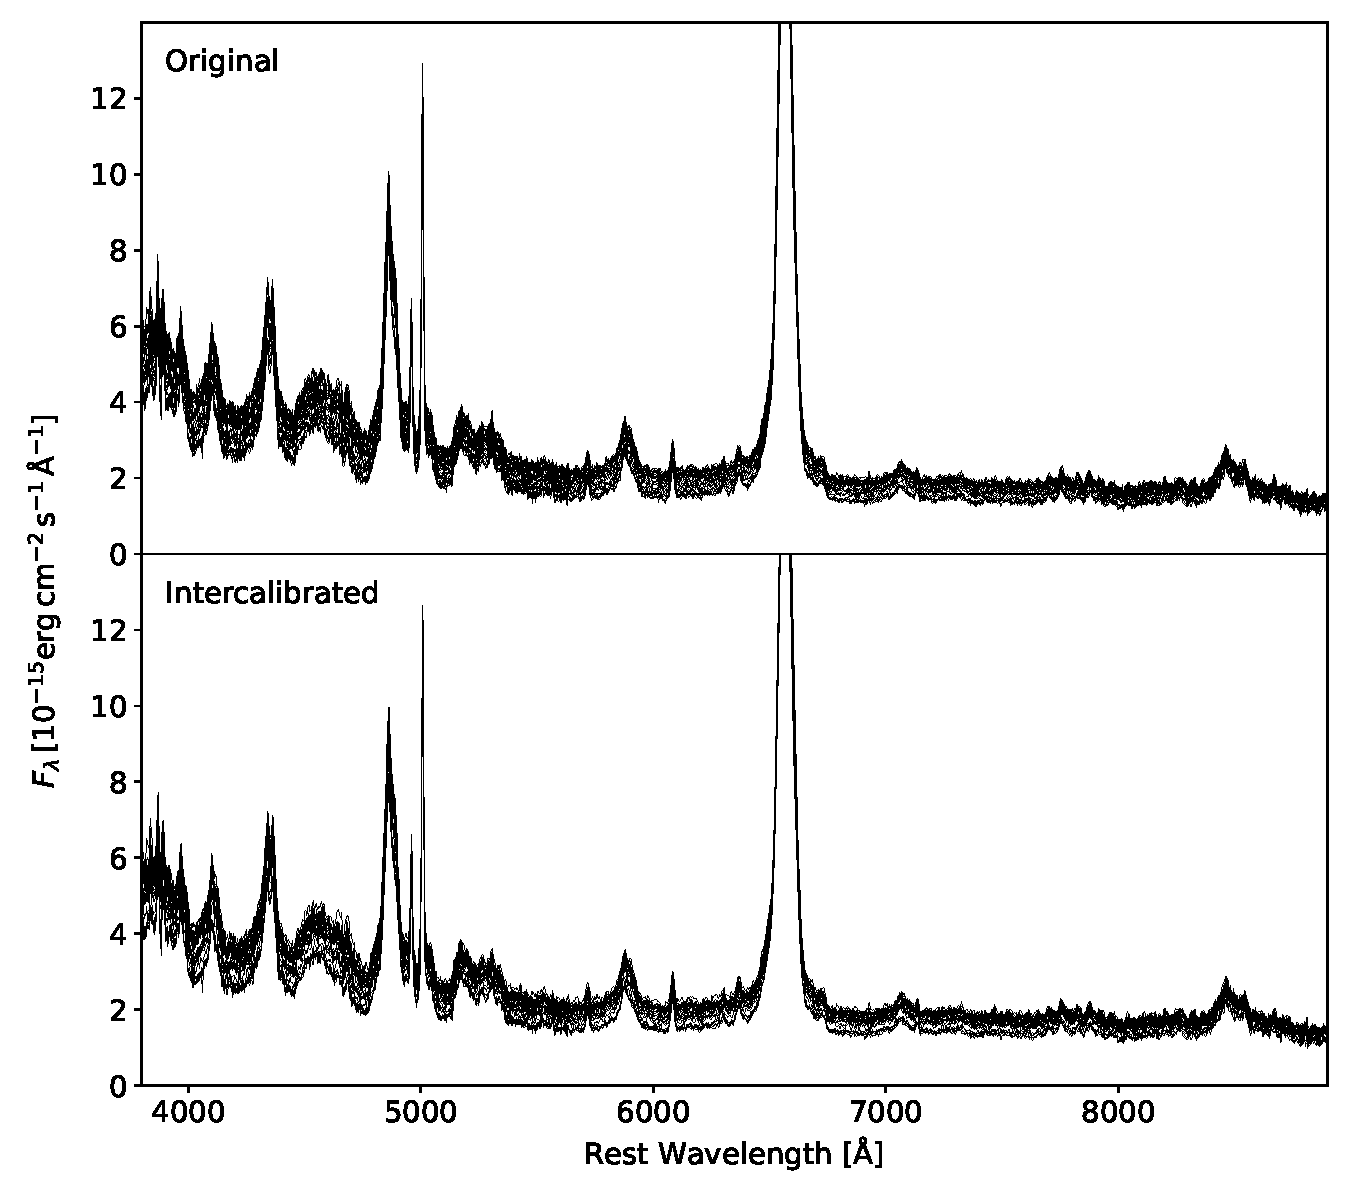
\includegraphics[width=0.7\textwidth]{pictures/Chapter3/comparison_spectra}
	\caption{Comparison of the optical spectral range of the original spectra and the [O \textsc{iii}] $\lambda5007$ intercalibrated spectra from the 2016 campaign of NGC 4593.}
	\label{fig:comparison_spectra}
\end{figure}




\begin{figure}[!ht]
	\centering
	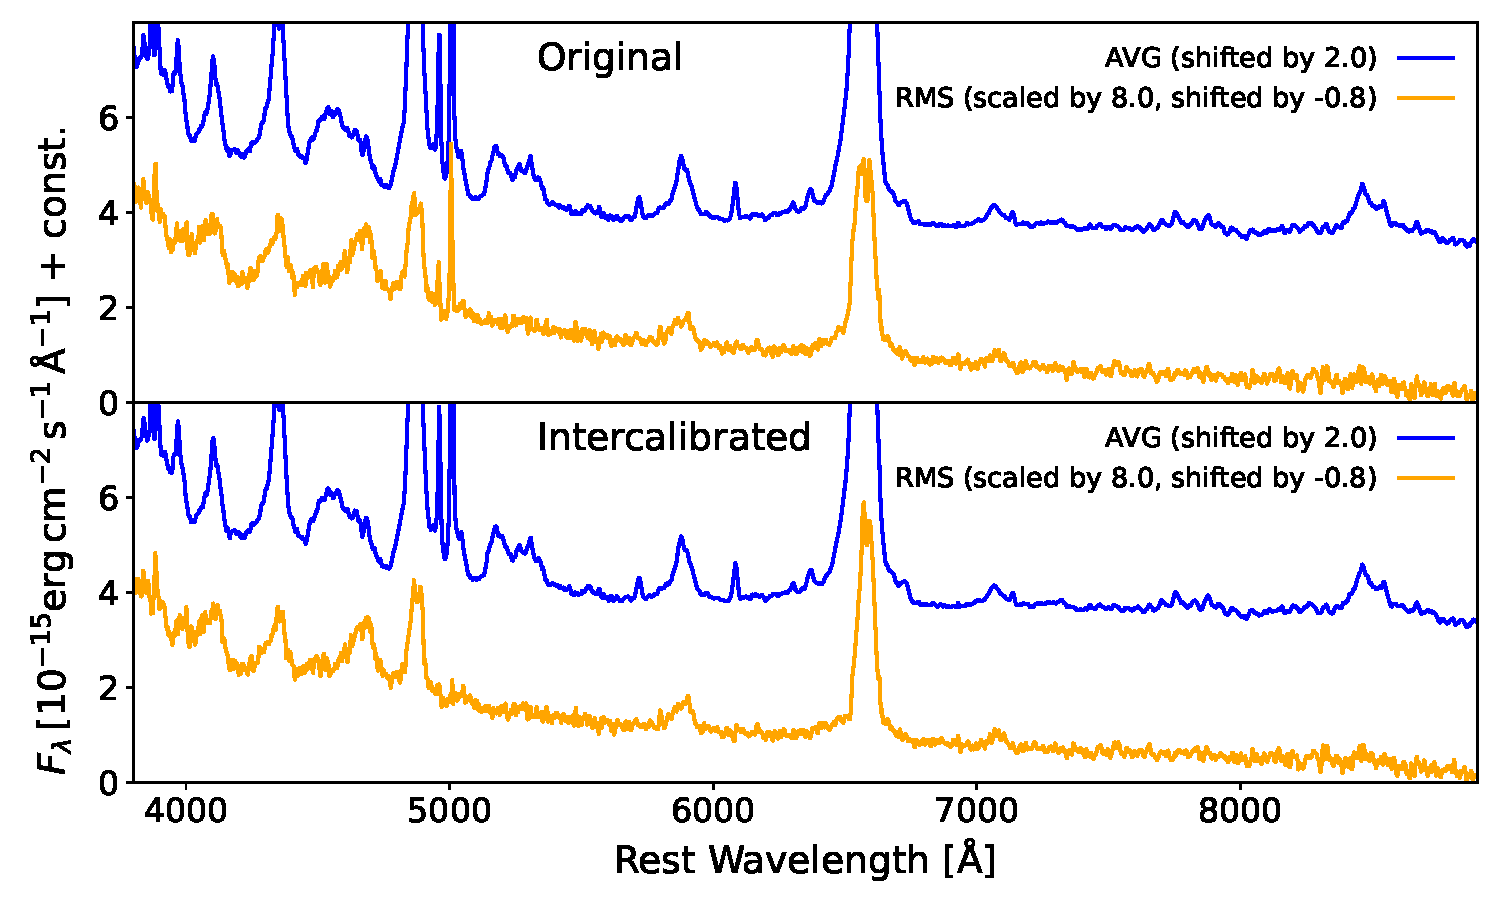
\includegraphics[width=0.7\textwidth]{pictures/Chapter3/comparison_avg_rms}
	\caption{Comparison of the optical spectral range of the avg and rms spectra from the original data and the [O \textsc{iii}] $\lambda5007$ intercalibrated data from the 2016 campaign of NGC 4593.}
	\label{fig:comparison_spectra_avg_rms}
\end{figure}



